\section{Results}
\label{results}
We apply our revised algorithm to HEG of several different $r_s$ values in the mid to high density region and both the 14-electron and the 54-electron supercell sizes.
In each case, we calculate the correlation energies in several basis sets of different momentum cutoffs, and perform a complete basis set (CBS) extrapolation in the end.

We notice that when the electron density is high, the correlation energies depends significantly on the momentum cutoff.
Hence, in order to obtain more accurate results, we use up to 39,886 orbitals in our calculations.
In the high density region, this decreases the CBS extrapolation distance in previous literature by about more than an order of magnitude, and thus give us much shorter extrapolation distances and more accurate results.

\subsection{14-Electron Supercell}
\begin{figure}
  \begin{center}
  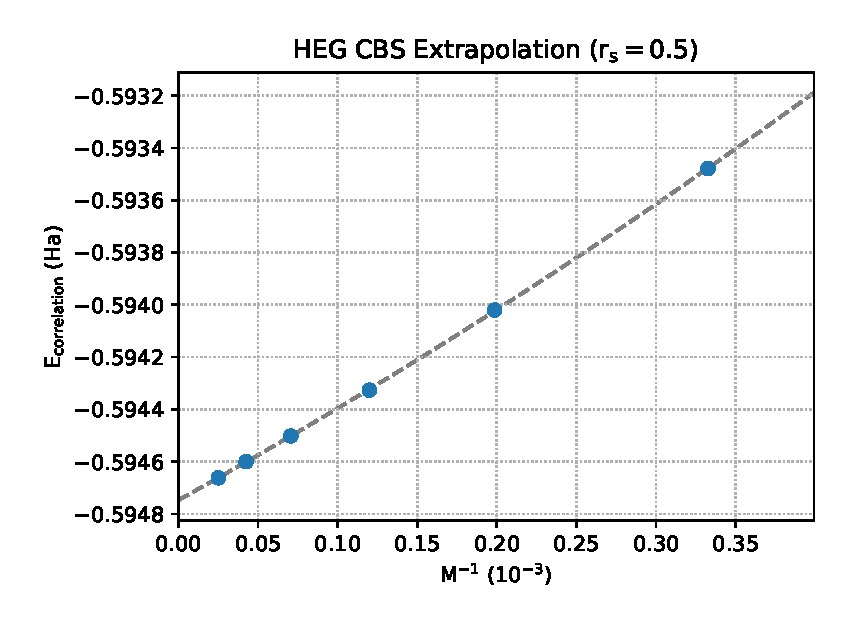
\includegraphics[width=\linewidth]{figs/cbs14e_05.eps}
  \end{center}
  \vspace{-0.2cm}
  \caption{Complete basis set extrapolation for HEG 14-electron supercell with $r_s=0.5$.
  The extrapolated correlation energy is $-0.594748(12)$~Ha.
  }
  \label{fig:cbs14e_05}
\end{figure}
\begin{figure}
  \begin{center}
  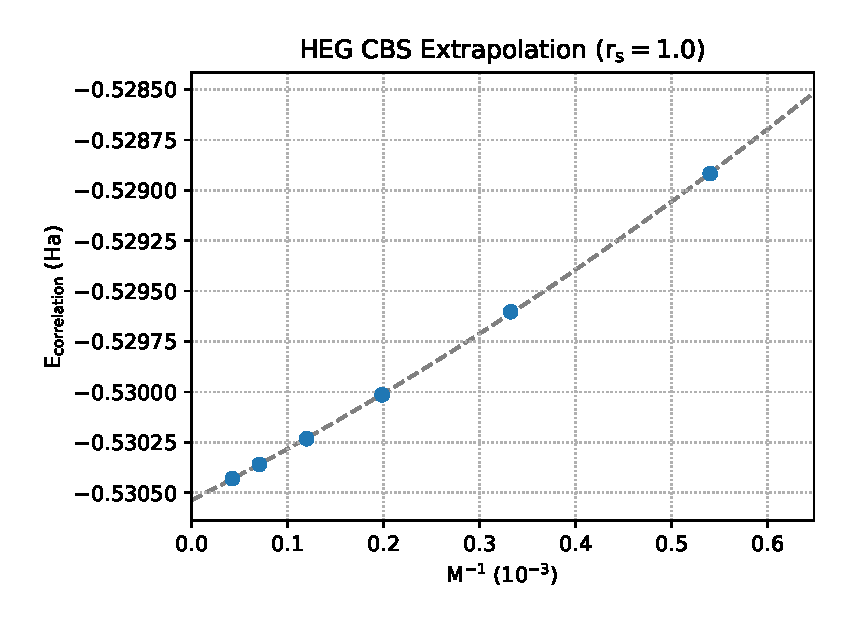
\includegraphics[width=\linewidth]{figs/cbs14e_10.eps}
  \end{center}
  \vspace{-0.2cm}
  \caption{Complete basis set extrapolation for HEG 14-electron supercell with $r_s=1.0$.
  The extrapolated correlation energy is $-0.530536(18)$~Ha.
  }
  \label{fig:cbs14e_10}
\end{figure}
\begin{figure}
  \begin{center}
  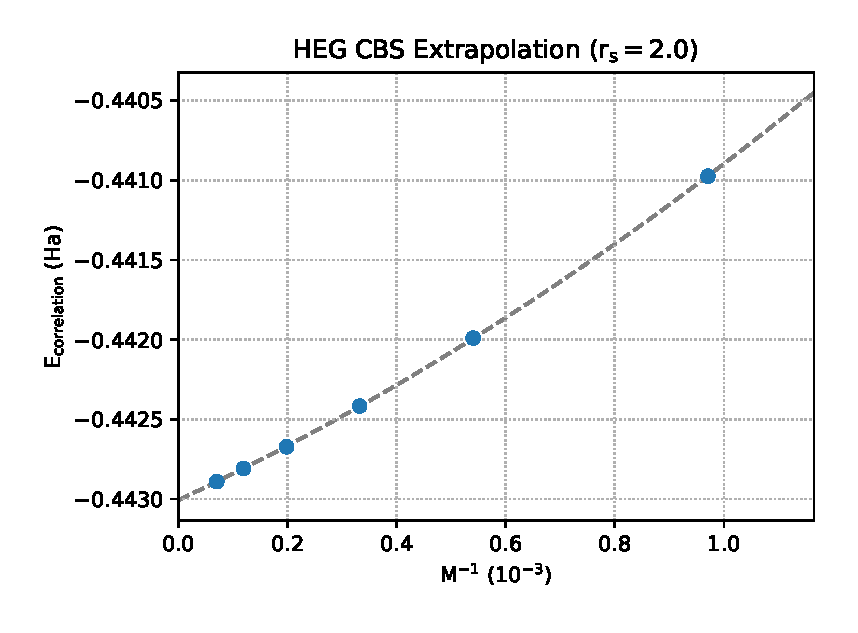
\includegraphics[width=\linewidth]{figs/cbs14e_20.eps}
  \end{center}
  \vspace{-0.2cm}
  \caption{Complete basis set extrapolation for HEG 14-electron supercell with $r_s=2.0$.
  The extrapolated correlation energy is $-0.443007(12)$~Ha.
  }
  \label{fig:cbs14e_20}
\end{figure}
\begin{figure}
  \begin{center}
  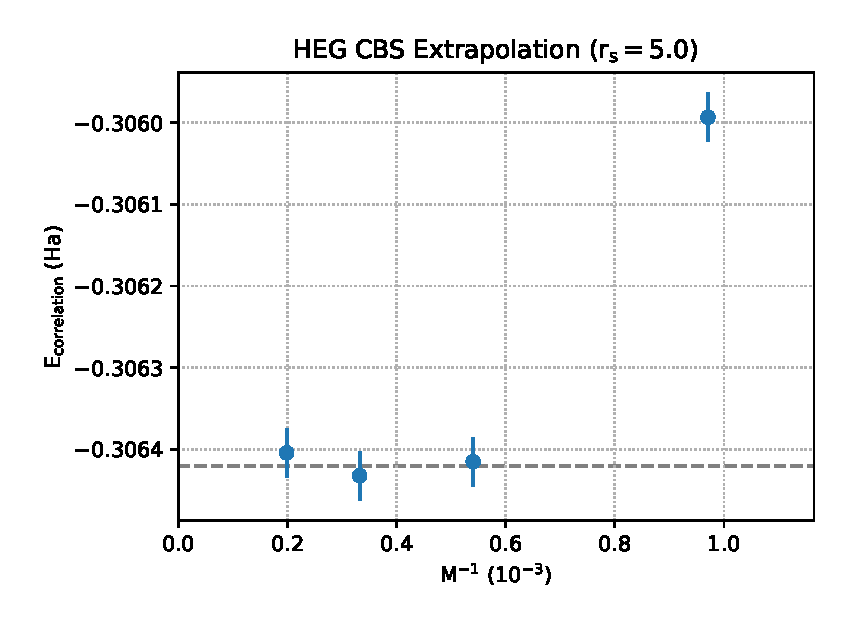
\includegraphics[width=\linewidth]{figs/cbs14e_50.eps}
  \end{center}
  \vspace{-0.2cm}
  \caption{Complete basis set extrapolation for HEG 14-electron supercell with $r_s=5.0$.
  Since the correlation energy is already converged after 2000 orbitals, we use the average of the last 3 points in this case.
  The extrapolated correlation energy is $-0.30642(5)$~Ha.
  }
  \label{fig:cbs14e_50}
\end{figure}
Fig.~\ref{fig:cbs14e_05} to \ref{fig:cbs14e_50} show our CBS extrapolation curves and Table~\ref{tab:results} reports our extrapolated correlation energies.
Here $M$ is the number of spin orbitals included in a plane wave basis set.

We use quadratic extrapolations weighted by $1/M$ for $r_s$ from 0.5 to 2.0.
For $r_s=5.0$, since it is already converged at the size of the basis sets that we use, we take the average of the last three points.
\begin{table}
\caption{Summary of the HEG Total Correlation Energies~(Ha).
CCMC~\cite{neufeld2017study} uses quantum Monte Carlo to evaluate coupled cluster wavefunctions with up to 1030 orbitals and 5\nth order excitation (CCSDTQ5).
FCIQMC~\cite{shepherd2012full} and its recent improvement FCIQMC-TC~\cite{luo2018combining} use up to 2368 orbitals.
SHCI uses up to 39886 orbitals, which give shorter extrapolation distances and much more accurate results than CCMC and FCIQMC.
}
\label{tab:results}
\begin{tabular}{| c || c || c | c | c | c |}
 \hline
 $r_s$ & SHCI & CCMC & FCIQMC & FCIQMC-TC \\
 \hline\hline
 0.5 & -0.594748(12) & -0.5947(2) & -0.5959(7) & -0.5948(2)\\
 \hline
 1.0 & -0.530536(18) & -0.5311(2) & -0.5316(4) & -0.5309(2)\\
 \hline
 2.0 & -0.443007(12) & -0.4434(10) & -0.444(1) & -0.4440(3)\\
 \hline
 5.0 & -0.30642(5) & -0.3025(4) & -0.307(1) & -0.3078(3)\\
 % DMC~\cite{rios2006inhomogeneous}
%  \hline
%  54 & 0.5 & -2.4316(6) & - & -2.435(7) & -2.387(2) \\
%  \hline
%  54 & 1.0 & -2.114(2) & - & -2.124(3) &  -2.125(2) \\
 \hline
\end{tabular}
\end{table}

We can see from this table that the results from SHCI are significantly more accurate than previous results.
This is mainly due to the fact that the high performance of SHCI and its capability to work with large basis sets enable us to go much closer to the infinite basis set. Fig.~\ref{fig:comparison} which plots the raw data points from FCIQMC~\cite{shepherd2012full} and SHCI, illustrates this.
\begin{figure}
  \begin{center}
  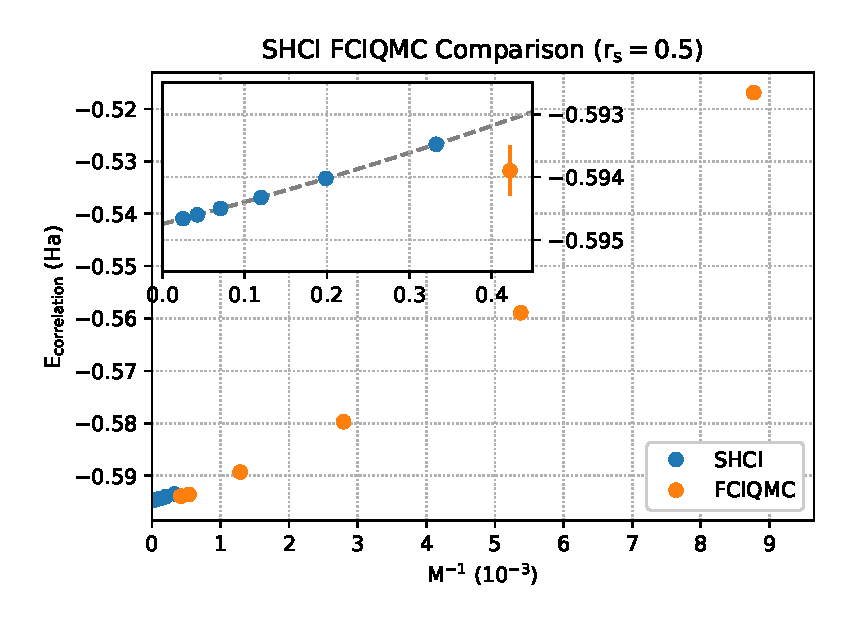
\includegraphics[width=\linewidth]{figs/compare.eps}
  \end{center}
  \vspace{-0.2cm}
  \caption{Comparison between SHCI results and FCIQMC results for $r_s=0.5$.
  Note that all the points have error bars smaller than the size of the points themselves except for the FCIQMC point on the zoomed-in view.
  SHCI goes much closer to the infinite basis set and thus achieves more accurate and reliable extrapolated results.
  }
  \label{fig:comparison}
\end{figure}

\subsection{54-Electron Supercell}
We also apply SHCI to the 54-electron supercell case.
Fig.~\ref{fig:cbs54e_05} shows the CBS extrapolation and Table~\ref{tab:results54} compares the SHCI results with FCIQMC and DMC.

We can see that our SHCI result agrees well with FCIQMC, but slighly lower than FCIQMC-TC, and all of them are much higher then BF-DMC, which probably used a poor trail wavefunction.
In these SHCI calculations, we use an order of magnitude more orbitals than FCIQMC and FCIQMC-TC, and the extrapolation distance of SHCI is about an order of magnitude smaller than FCIQMC and 4 times smaller than FCIQMC-TC.
Hence, we believe the extrapolated value from SHCI is likely to be more accurate and reliable than both FCIQMC and FCIQMC-TC.

\begin{figure}
  \begin{center}
  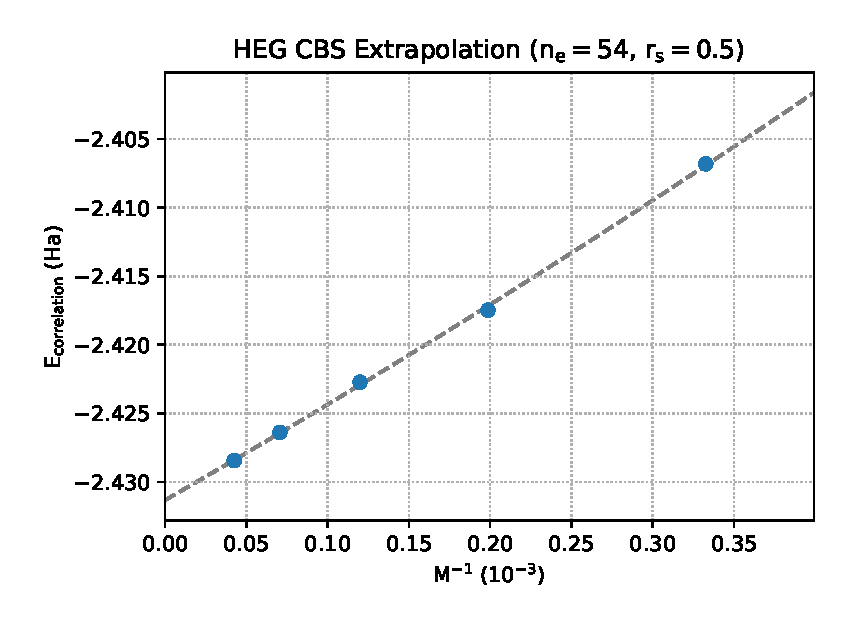
\includegraphics[width=\linewidth]{figs/cbs54e_05.eps}
  \end{center}
  \vspace{-0.2cm}
  \caption{Complete basis set extrapolation for HEG 54-electron supercell with $r_s=0.5$.
  The extrapolated correlation energy is $-2.4313(11)$~Ha.
  }
  \label{fig:cbs54e_05}
\end{figure}
\begin{table}
\caption{Summary of the HEG Total Correlation Energies~(Ha) with 54-Electron Supercells.
DMC~\cite{rios2006inhomogeneous} uses real space basis and backflow wave function.
FCIQMC~\cite{shepherd2012full} and its recent improvement FCIQMC-TC~\cite{luo2018combining} use up to 1850 orbitals.
SHCI uses up to 23506 orbitals, which give much shorter extrapolation distances than FCIQMC and thus more accurate results.
}
\label{tab:results54}
\begin{tabular}{| c || c || c | c | c | c |}
 \hline
 $r_s$ & SHCI & FCIQMC & FCIQMC-TC & BF-DMC \\
 \hline\hline
 0.5 & -2.4313(11) & -2.435(7) & -2.425(1) & -2.387(2) \\
 \hline
 % DMC~\cite{rios2006inhomogeneous}
%  \hline
%  54 & 0.5 & -2.4316(6) & - & -2.435(7) & -2.387(2) \\
%  \hline
%  54 & 1.0 & -2.114(2) & - & -2.124(3) &  -2.125(2) \\
 \hline
\end{tabular}
\end{table}